
\section{Auswertung}
\label{sec:Auswertung}
Die Graphen in Abbildung \ref{fig:rund} bis \ref{fig:beidseitiglinear2} wurden jeweils sowohl mit Matplotlib \cite{matplotlib} als auch NumPy \cite{numpy} erstellt. Die Fehlerrechnung wurde mit Unterstützung von Uncertainties \cite{uncertainties} durchgeführt.\newline 
Die Gewichtskraft $F$ kann mit $g=\SI{9.81}{\newton\per\kilogram}$ \cite{g} berechnet werden durch:
\begin{equation}
	F = m \cdot g \text{.} \label{Gewichtskraft}
\end{equation}

\subsection{Bestimmung des Elastizitätsmoduls über die Biegung eines runden, einseitig eingespannten Stabes}
\begin{figure}
	\centering
	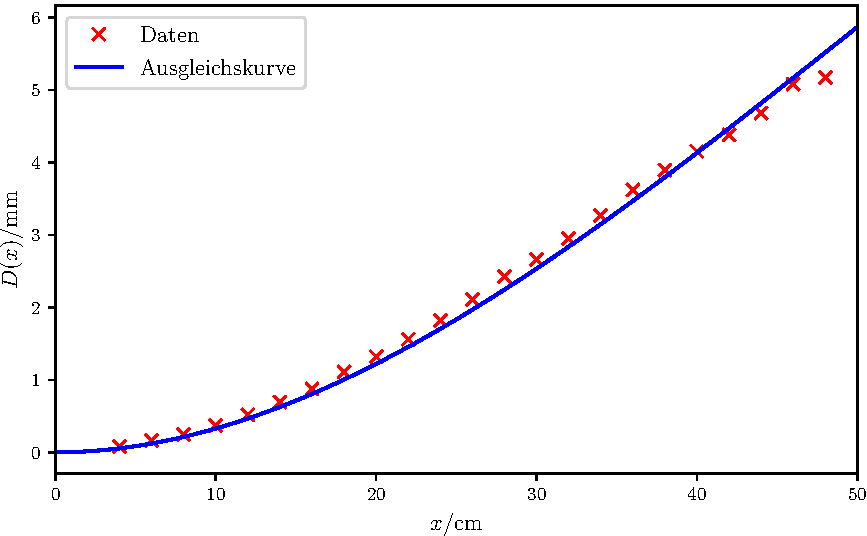
\includegraphics[width=\linewidth-70pt,height=\textheight-70pt,keepaspectratio]{content/images/StabRundEinseitig1.pdf}
	\caption{Die gemessene Auslenkung $D(x)$ des runden, einseitig eingespannten Stabes in Abhängigkeit des horizontalen Abstandes zum fixierten Ende.}
	\label{fig:rund}
\end{figure}
\begin{figure}
	\centering
	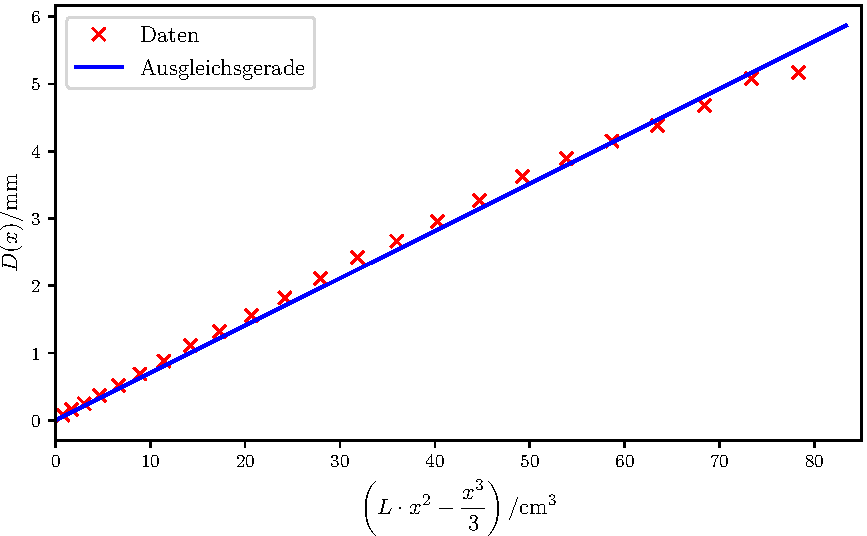
\includegraphics[width=\linewidth-70pt,height=\textheight-70pt,keepaspectratio]{content/images/StabRundEinseitig2.pdf}
	\caption{Die gemessene Auslenkung $D(x)$ des runden, einseitig eingespannten Stabes in Abhängigkeit des horizontalen Abstandes zum fixierten Ende in linearisierter Darstellung.}
	\label{fig:rundlinear}
\end{figure}
\begin{table}
	\caption{Die gemessene Auslenkung $D(x)$ des einseitig eingespannten, runden Stabes an den jeweiligen horizontalen Abständen $x$ zum fixierten Ende.}
	\begin{minipage}{0.5\textwidth}
		\centering
		\label{tab:tabStabRundEinseitig1}
	\sisetup{table-format=1.2}
	\begin{tabular}{S[table-format=2.1]S[table-format=1.2]}
		\toprule
		{$x/\si{\centi\meter}$} & {$D(x)/\si{\milli\meter}$} \\
		\midrule
		4.0 & 0.08 \\
		6.0 & 0.16 \\
		8.0 & 0.25 \\
		10.0 & 0.37 \\
		12.0 & 0.52 \\
		14.0 & 0.69 \\
		16.0 & 0.88 \\
		18.0 & 1.11 \\
		20.0 & 1.32 \\
		22.0 & 1.56 \\
		24.0 & 1.82 \\
		\bottomrule
	\end{tabular}

	\end{minipage}
	\begin{minipage}{0.5\textwidth}
		\centering
		\label{tab:tabStabRundEinseitig2}
	\sisetup{table-format=1.2}
	\begin{tabular}{S[table-format=2.1]S[table-format=1.2]}
		\toprule
		{$x/\si{\centi\meter}$} & {$D(x)/\si{\milli\meter}$} \\
		\midrule
		26.0 & 2.11 \\
		28.0 & 2.42 \\
		30.0 & 2.66 \\
		32.0 & 2.95 \\
		34.0 & 3.27 \\
		36.0 & 3.62 \\
		38.0 & 3.89 \\
		40.0 & 4.15 \\
		42.0 & 4.38 \\
		44.0 & 4.68 \\
		46.0 & 5.08 \\
		48.0 & 5.17 \\
		\bottomrule
	\end{tabular}

	\end{minipage}
\end{table}
Die Ausgleichskurve in Abbildung \ref{fig:rund} besitzt die Form $y = a ( L x^2 - \frac{x^3}{3} ) $ und die Ausgleichsgerade in Abbildung \ref{fig:rundlinear} die Form $y=a x$. Aus Formel \eqref{eq:??} ergibt sich das Flächenträgheitsmoment $I_.{Kreis}$ des runden Stabes  zu $\SI{4.91e-10}{\metre\tothe{4}}$. Die Kraft F berechnet sich aus dem angehängtem Gewicht von $\SI{522e-3}{\kilogram}$ mit Formel \eqref{Gewichtskraft} zu $\SI{5.12}{\newton}$. Eine nicht lineare Ausgleichsrechnung der Form $y = a ( L x^2 - \frac{x^3}{3})$ liefert mit der gemessenen Länge $L$ von $\SI{50.0e-2}{\metre}$ und den Wertepaaren aus Tabelle \ref{tab:tabStabRundEinseitig1} nach Formel \eqref{eq:??}:
\begin{displaymath}
	E = \SI{7.41(7)e10}{\pascal}\text{.}
\end{displaymath}
%Die linearisierte Darstellung in \ref{fig:rundlinear} belegt die Richtigkeit der vorangegangenen, theoretischen Überlegungen.

\subsection{Bestimmung des Elastizitätsmoduls über die Biegung eines quadratischen, einseitig eingespannten Stabes}\label{subsec:QuadratischEinseitig}

\begin{figure}
	\centering
	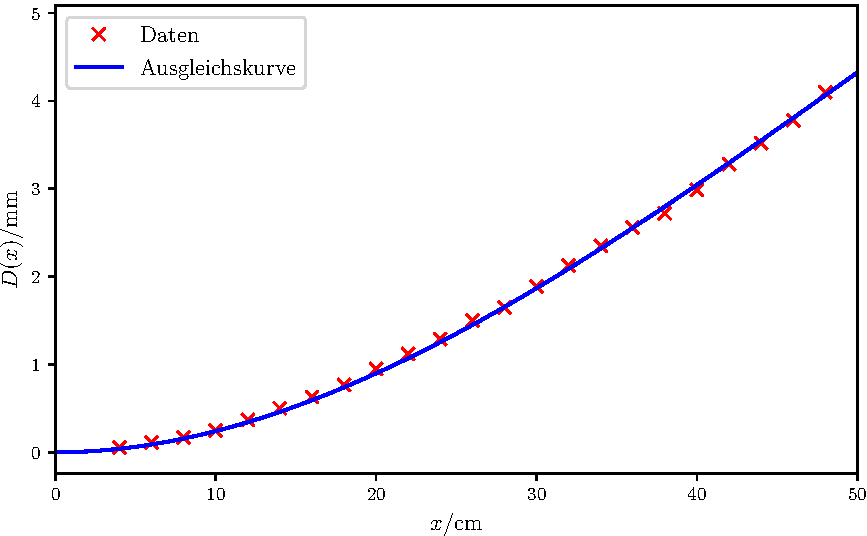
\includegraphics[width=\linewidth-70pt,height=\textheight-70pt,keepaspectratio]{content/images/StabQuadratEinseitig1.pdf}
	\caption{Die gemessene Auslenkung $D(x)$ des quadratischen, einseitig eingespannten Stabes in Abhängigkeit des horizontalen Abstandes zum fixierten Ende.}
	\label{fig:quadratisch}
\end{figure}
\begin{figure}
	\centering
	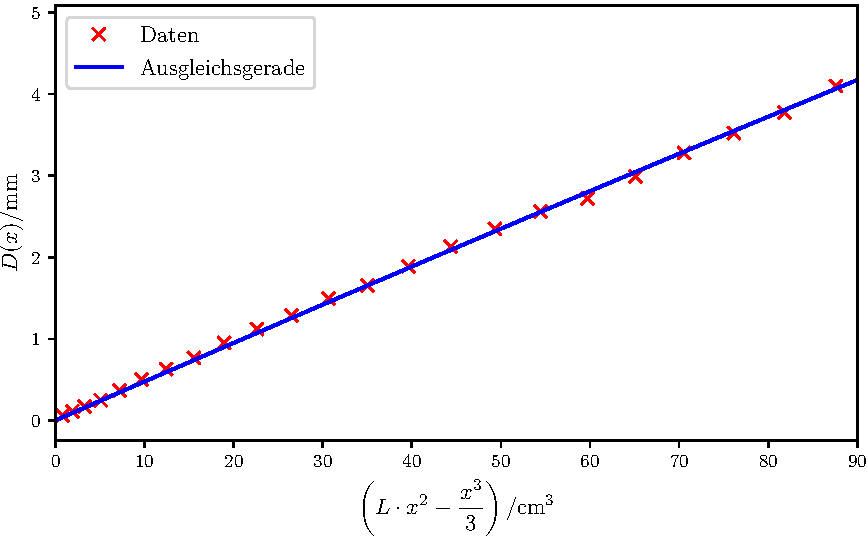
\includegraphics[width=\linewidth-70pt,height=\textheight-70pt,keepaspectratio]{content/images/StabQuadratEinseitig2.pdf}
	\caption{Die gemessene Auslenkung $D(x)$ des quadratischen, einseitig eingespannten Stabes in Abhängigkeit des horizontalen Abstandes zum fixierten Ende in linearisierter Darstellung.}
	\label{fig:quadratischlinear}
\end{figure}
\begin{table}
	\caption{Die gemessene Auslenkung $D(x)$ des einseitig eingespannten, quadratischen Stabes an den jeweiligen horizontalen Abständen $x$ zum fixierten Ende.}
	\begin{minipage}{0.5\textwidth}
		\centering
		\label{tab:tabStabQuadratEinseitig1}
	\sisetup{table-format=1.2}
	\begin{tabular}{S[table-format=2.1]S[table-format=1.2]}
		\toprule
		{$x/\si{\centi\meter}$} & {$D(x)/\si{\milli\meter}$} \\
		\midrule
		4.0 & 0.06 \\
		6.0 & 0.11 \\
		8.0 & 0.17 \\
		10.0 & 0.25 \\
		12.0 & 0.37 \\
		14.0 & 0.50 \\
		16.0 & 0.63 \\
		18.0 & 0.77 \\
		20.0 & 0.95 \\
		22.0 & 1.12 \\
		24.0 & 1.29 \\
		\bottomrule
	\end{tabular}

	\end{minipage}
	\begin{minipage}{0.5\textwidth}
		\centering
		\label{tab:tabStabQuadratEinseitig2}
	\sisetup{table-format=1.2}
	\begin{tabular}{S[table-format=2.1]S[table-format=1.2]}
		\toprule
		{$x/\si{\centi\meter}$} & {$D(x)/\si{\milli\meter}$} \\
		\midrule
		26.0 & 1.50 \\
		28.0 & 1.65 \\
		30.0 & 1.89 \\
		32.0 & 2.13 \\
		34.0 & 2.35 \\
		36.0 & 2.56 \\
		38.0 & 2.72 \\
		40.0 & 2.99 \\
		42.0 & 3.28 \\
		44.0 & 3.52 \\
		46.0 & 3.78 \\
		48.0 & 4.10 \\
		\bottomrule
	\end{tabular}

	\end{minipage}
\end{table}
Die Ausgleichskurve in Abbildung \ref{fig:quadratisch} besitzt die Form $y = a ( L x^2 - \frac{x^3}{3} ) $ und die Ausgleichsgerade in Abbildung \ref{fig:quadratischlinear} die Form $y=a x$. Aus Formel \eqref{eq:??} ergibt sich das Flächenträgheitsmoment $I_.{Quadrat}$ des quadratischen Stabes zu $\SI{8.33e-10}{\metre\tothe{4}}$. Die Kraft F berechnet sich aus dem angehängtem Gewicht von $\SI{540,93e-3}{\kilogram}$ mit Formel \eqref{Gewichtskraft} zu $\SI{5.30}{\newton}$. Eine nicht lineare Ausgleichsrechnung der Form $y = a ( L x^2 - \frac{x^3}{3})$ liefert mit der gemessenen Länge $L$ von $\SI{54.0e-2}{\metre}$ und den Wertepaaren aus Tabelle \ref{tab:tabStabQuadratEinseitig1} nach Formel \eqref{eq:??}:
\begin{displaymath}
E = \SI{6.13(2)e10}{\pascal}\text{.}
\end{displaymath}
% Die Theorie wird wieder bestätigt.

\subsection{Bestimmung des Elastizitätsmoduls über die Biegung eines quadratischen, beidseitig aufgelegten Stabes}

\begin{figure}
	\centering
	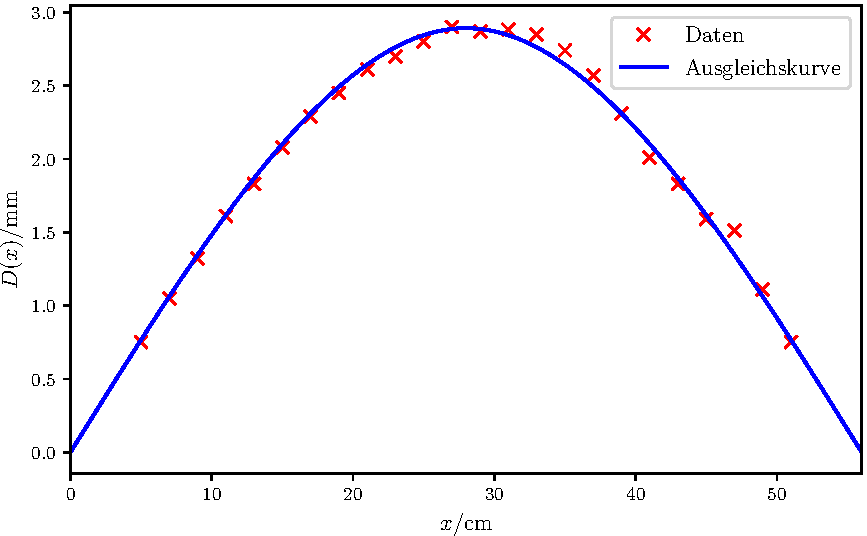
\includegraphics[width=\linewidth-70pt,height=\textheight-70pt,keepaspectratio]{content/images/StabQuadratBeidseitig1.pdf}
	\caption{Die gemessene Auslenkung $D(x)$ des quadratischen, beidseitig aufliegenden Stabes in Abhängigkeit des horizontalen Abstandes zum rechten Auflagepunkt.}
	\label{fig:beidseitig}
\end{figure}
\begin{figure}
	\centering
	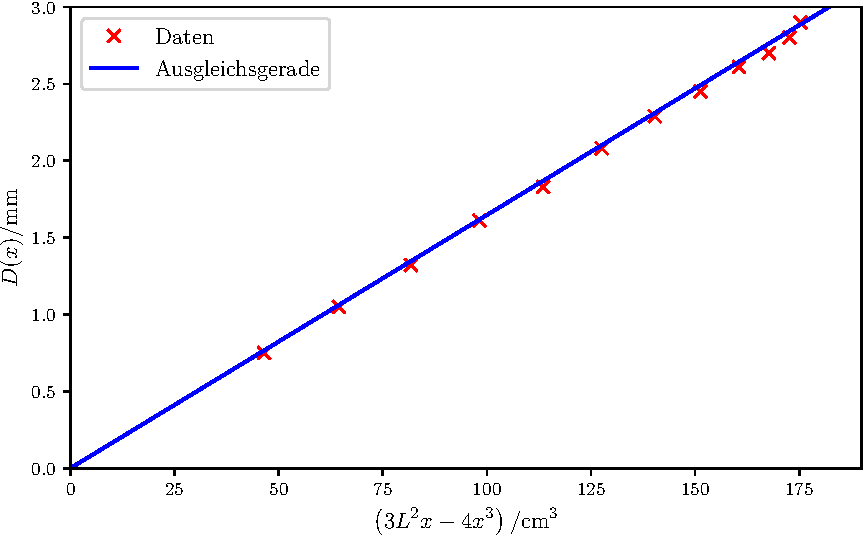
\includegraphics[width=\linewidth-70pt,height=\textheight-70pt,keepaspectratio]{content/images/StabQuadratBeidseitig2.pdf}
	\caption{Die gemessene Auslenkung $D(x)$ des quadratischen, beidseitig aufliegenden Stabes von der rechten Seite bis zur Stabmitte in Abhängigkeit des horizontalen Abstandes zum rechten Auflagepunkt in linearisierter Form.}
	\label{fig:beidseitiglinear1}
\end{figure}
\begin{figure}
	\centering
	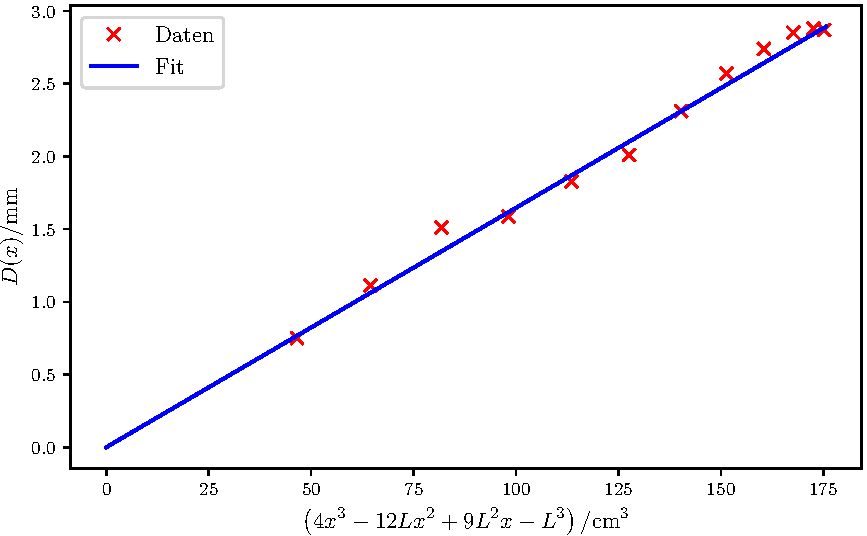
\includegraphics[width=\linewidth-70pt,height=\textheight-70pt,keepaspectratio]{content/images/StabQuadratBeidseitig3.pdf}
	\caption{Die gemessene Auslenkung $D(x)$ des quadratischen, beidseitig aufliegenden Stabes von der linken Seite bis zur Stabmitte in Abhängigkeit des horizontalen Abstandes zum rechten Auflagepunkt in linearisierter Form.}
	\label{fig:beidseitiglinear2}
\end{figure}
\begin{table}
	\caption{Die gemessene Auslenkung $D(x)$ des beidseitig aufliegenden, quadratischen Stabes an den jeweiligen horizontalen Abständen $x$ zum rechten Auflagepunkt.}
	\begin{minipage}[c]{0.5\textwidth}
		\centering
		\label{tab:tabStabQuadratBeidseitig1}
	\sisetup{table-format=1.2}
	\begin{tabular}{S[table-format=2.1]S[table-format=1.2]}
		\toprule
		{$x/\si{\centi\meter}$} & {$D(x)/\si{\milli\meter}$} \\
		\midrule
		5.0 & 0.75 \\
		7.0 & 1.05 \\
		9.0 & 1.32 \\
		11.0 & 1.61 \\
		13.0 & 1.83 \\
		15.0 & 2.08 \\
		17.0 & 2.29 \\
		19.0 & 2.45 \\
		21.0 & 2.61 \\
		23.0 & 2.70 \\
		25.0 & 2.80 \\
		27.0 & 2.90 \\
		\bottomrule
	\end{tabular}

	\end{minipage}
	\begin{minipage}[c]{0.5\textwidth}
		\centering
		\label{tab:tabStabQuadratBeidseitig2}
	\sisetup{table-format=1.2}
	\begin{tabular}{S[table-format=2.1]S[table-format=1.2]}
		\toprule
		{$x/\si{\centi\meter}$} & {$D(x)/\si{\milli\meter}$} \\
		\midrule
		29.0 & 2.87 \\
		31.0 & 2.88 \\
		33.0 & 2.85 \\
		35.0 & 2.74 \\
		37.0 & 2.57 \\
		39.0 & 2.31 \\
		41.0 & 2.01 \\
		43.0 & 1.83 \\
		45.0 & 1.59 \\
		47.0 & 1.51 \\
		49.0 & 1.11 \\
		51.0 & 0.75 \\
		\bottomrule
	\end{tabular}

	\end{minipage}
\end{table}
Die Ausgleichskurve in Abbildung \ref{fig:beidseitig} besitzt die Form:
\begin{equation}
	y =
	\begin{cases}
	a\left(3L^2 x-4x^3\right)& \text{für }0\leq x \leq \frac{L}{2} \\
	a\left(4 x^3 -12 L x^2 + 9 L^2 x -L 3 \right)& \text{für }\frac{L}{2} < x \leq L
	\end{cases} \label{FunktionBeidseitig}
\end{equation}
Die Ausgleichsgeraden in den Abbildungen \ref{fig:beidseitiglinear1} und \ref{fig:beidseitiglinear2} besitzen die Form $y=a x$.
Das Flächenträgheitsmoment $I_.{Quadrat}$ des quadratischen Stabes ist aus Abschnitt \ref{subsec:QuadratischEinseitig} bekannt.  Die Kraft F berechnet sich aus dem angehängtem Gewicht von $\SI{4711e-3}{\kilogram}$ mit Formel \eqref{Gewichtskraft} zu $\SI{46.20}{\newton}$. Eine nicht lineare Ausgleichsrechnung der Form \eqref{FunktionBeidseitig} liefert mit der gemessenen Länge $L$ von $\SI{56.0e-2}{\metre}$ und den Wertepaaren aus Tabelle \ref{tab:tabbeidseitig1} nach Formel \eqref{eq:??} und \eqref{eq:??}:
\begin{displaymath}
E = \SI{7.01(4)e10}{\pascal}\text{.}
\end{displaymath}
%Auch hier zeigen die Graphen das vorhergesagte Verhalten auf.
